\par
\section{Driver programs for the {\tt Graph} object}
\label{section:Graph:drivers}
\par
This section contains brief descriptions of six driver programs.
\par
%=======================================================================
\begin{enumerate}
%-----------------------------------------------------------------------
\item
\begin{verbatim}
checkComponents msglvl msgFile inGraphFile 
\end{verbatim}
This driver program reads in a {\tt Graph} object from a file,
and prints out information about the number of vertices and weights
of the vertices in the components.
\begin{itemize}
\item
The {\tt msglvl} parameter determines the amount of output ---
taking {\tt msglvl >= 3} means that all objects are written
to the message file.
\item
The {\tt msgFile} parameter determines the message file --- if {\tt
msgFile} is {\tt stdout}, then the message file is {\it stdout},
otherwise a file is opened with {\it append} status to receive any
output data.
\item
The {\tt inGraphFile} parameter is the input file for the {\tt Graph}
object. It must be of the form {\tt *.graphf} or {\tt *.graphb}.
The {\tt Graph} object is read from the file via the
{\tt Graph\_readFromFile()} method.
\end{itemize}
%-----------------------------------------------------------------------
\item
\begin{verbatim}
compressGraph msglvl msgFile inGraphFile coarseType outMapFile outGraphFile
\end{verbatim}
This driver program reads in a {\tt Graph} object from a file,
computes the equivalence map to its natural compressed graph
(the first graph need not be unit weight), and constructs the
natural compressed graph.
The equivalence map and compressed graph are optionally written out
to files.
\begin{itemize}
\item
The {\tt msglvl} parameter determines the amount of output ---
taking {\tt msglvl >= 3} means that all objects are written
to the message file.
\item
The {\tt msgFile} parameter determines the message file --- if {\tt
msgFile} is {\tt stdout}, then the message file is {\it stdout},
otherwise a file is opened with {\it append} status to receive any
output data.
\item
The {\tt inGraphFile} parameter is the input file for the {\tt Graph}
object. It must be of the form {\tt *.graphf} or {\tt *.graphb}.
The {\tt Graph} object is read from the file via the
{\tt Graph\_readFromFile()} method.
\item
The {\tt coarseType} parameter defines the type of compressed
graph; valid values are in {\tt [0,3]}.
\item
The {\tt outMapFile} parameter is the output file for the {\tt IV}
object that holds the equivalence map.
If {\tt outMapFile} is {\tt none} then the {\tt IV} object is not
written to a file. 
Otherwise, the {\tt IV\_writeToFile()} method is called to write
the {\tt IV} object to 
a formatted file (if {\tt outMapFile} is of the form {\tt *.ivf}),
or
a binary file (if {\tt outMapFile} is of the form {\tt *.ivb}).
\item
The {\tt outGraphFile} parameter is the output file for the 
compressed {\tt Graph} object. 
If {\tt outGraphFile} is {\tt none} then the {\tt Graph} object is not
written to a file. 
Otherwise, the {\tt Graph\_writeToFile()} method is called to write
the graph to 
a formatted file (if {\tt outGraphFile} is of the form {\tt *.graphf}),
or
a binary file (if {\tt outGraphFile} is of the form {\tt *.graphb}).
\end{itemize}
%-----------------------------------------------------------------------
\item
\begin{verbatim}
expandGraph msglvl msgFile inGraphFile inMapFile outGraphFile
\end{verbatim}
This driver program reads in a {\tt Graph} object and a map {\tt
IV} object from two files.
It then creates a new {\tt Graph} object which is the original
graph ``expanded'' by the map, and optionally writes this object
to a file.
The program {\tt expandGraph} is the inverse of {\tt compressGraph}.
\begin{itemize}
\item
The {\tt msglvl} parameter determines the amount of output ---
taking {\tt msglvl >= 3} means that all objects are written
to the message file.
\item
The {\tt msgFile} parameter determines the message file --- if {\tt
msgFile} is {\tt stdout}, then the message file is {\it stdout},
otherwise a file is opened with {\it append} status to receive any
output data.
\item
The {\tt inGraphFile} parameter is the input file for the {\tt Graph}
object. It must be of the form {\tt *.graphf} or {\tt *.graphb}.
The {\tt Graph} object is read from the file via the
{\tt Graph\_readFromFile()} method.
\item
The {\tt inMapFile} parameter is the input file for the {\tt IV}
object that holds the expansion map.
The {\tt IV\_readFromFile()} method is called to read
the map from 
a formatted file (if {\tt inMapFile} is of the form {\tt *.ivf}),
or
a binary file (if {\tt inMapFile} is of the form {\tt *.ivb}).
\item
The {\tt outGraphFile} parameter is the output file for the 
compressed {\tt Graph} object. 
If {\tt outGraphFile} is {\tt none} then the {\tt Graph} object is not
written to a file. 
Otherwise, the {\tt Graph\_writeToFile()} method is called to write
the graph to 
a formatted file (if {\tt outGraphFile} is of the form {\tt *.graphf}),
or
a binary file (if {\tt outGraphFile} is of the form {\tt *.graphb}).
\end{itemize}
%-----------------------------------------------------------------------
\item
\begin{verbatim}
mkGridGraph msglvl msgFile stencil n1 n2 n3 outFile 
\end{verbatim}
This driver program creates a Graph object for a finite difference
operator on a ${\tt n1} \times {\tt n2} \times {\tt n3}$ regular grid.
\begin{itemize}
\item
The {\tt msglvl} parameter determines the amount of output ---
taking {\tt msglvl >= 3} means that all objects are written
to the message file.
\item
The {\tt msgFile} parameter determines the message file --- if {\tt
msgFile} is {\tt stdout}, then the message file is {\it stdout},
otherwise a file is opened with {\it append} status to receive any
output data.
\item
Valid {\tt stencil} values are 
{\tt 5} for a 2-D 5-point operator,
{\tt 7} for a 3-D 7-point operator,
{\tt 9} for a 2-D 9-point operator,
{\tt 13} for a 2-D 13-point operator
and
{\tt 27} for a 3-D 27-point operator.
\item
{\tt n1} is the number of points in the first direction.
\item
{\tt n2} is the number of points in the second direction.
\item
{\tt n3} is the number of points in the third direction,
ignored for {\tt stencil} = {\tt 5}, {\tt 9} and {\tt 13}.
\item
The {\tt Graph} object is written to file {\tt outFile}.
It must be of the form {\tt *.graphf} or {\tt *.graphb}.
The {\tt Graph} object is written to the file via the
{\tt Graph\_writeToFile()} method.
\end{itemize}
%-----------------------------------------------------------------------
\item
\begin{verbatim}
testIO msglvl msgFile inFile outFile
\end{verbatim}
This driver program reads in a {\tt Graph} object from {\tt inFile}
and writes out the object to {\tt outFile}
\par
\begin{itemize}
\item
The {\tt msglvl} parameter determines the amount of output ---
taking {\tt msglvl >= 3} means the {\tt Graph} object is written
to the message file.
\item
The {\tt msgFile} parameter determines the message file --- if {\tt
msgFile} is {\tt stdout}, then the message file is {\it stdout},
otherwise a file is opened with {\it append} status to receive any
output data.
\item
The {\tt inFile} parameter is the input file for the {\tt Graph}
object. It must be of the form {\tt *.graphf} or {\tt *.graphb}.
The {\tt Graph} object is read from the file via the
{\tt Graph\_readFromFile()} method.
\item
The {\tt outFile} parameter is the output file for the {\tt Graph}
object. It must be of the form {\tt *.graphf} or {\tt *.graphb}.
The {\tt Graph} object is written to the file via the
{\tt Graph\_writeToFile()} method.
\end{itemize}
%-----------------------------------------------------------------------
\item
\begin{verbatim}
testIsSymmetric msglvl msgFile inFile 
\end{verbatim}
This driver program reads in a {\tt Graph} object and tests whether
it is symmetric using the {\tt Graph\_isSymmetric()} method.
This was useful in one application where the {\tt Graph} object was
constructed improperly.
\par
\begin{itemize}
\item
The {\tt msglvl} parameter determines the amount of output ---
taking {\tt msglvl >= 3} means the {\tt Graph} object is written
to the message file.
\item
The {\tt msgFile} parameter determines the message file --- if {\tt
msgFile} is {\tt stdout}, then the message file is {\it stdout},
otherwise a file is opened with {\it append} status to receive any
output data.
\item
The {\tt inFile} parameter is the input file for the {\tt Graph}
object. It must be of the form {\tt *.graphf} or {\tt *.graphb}.
The {\tt Graph} object is read from the file via the
{\tt Graph\_readFromFile()} method.
\end{itemize}
%-----------------------------------------------------------------------
\item
\begin{verbatim}
testWirebasket msglvl msgFile inGraphFile inStagesFile
               outStagesFile radius
\end{verbatim}
This driver program reads in a {\tt Graph} object and 
and a file that contains the stages ids of the vertices,
(stage equal to zero means the vertex is in the Schur complement),
and overwrites the stages vector to specify the stage that the
vertex lies for a wirebasket domain decomposition of the graph.
For a Schur complement vertex, its stage is precisely the number of
domains that lie within {\tt radius} edges of it.
The new stages vector is written to the {\tt outStagesFile} file.
\par
\begin{itemize}
\item
The {\tt msglvl} parameter determines the amount of output ---
taking {\tt msglvl >= 3} means the {\tt Graph} object is written
to the message file.
\item
The {\tt msgFile} parameter determines the message file --- if {\tt
msgFile} is {\tt stdout}, then the message file is {\it stdout},
otherwise a file is opened with {\it append} status to receive any
output data.
\item
The {\tt inGraphFile} parameter is the input file for the {\tt Graph}
object. It must be of the form {\tt *.graphf} or {\tt *.graphb}.
The {\tt Graph} object is read from the file via the
{\tt Graph\_readFromFile()} method.
\item
The {\tt inStagesFile} parameter is the input file for the {\tt IV}
object that holds the component ids. 
It must be of the form {\tt *.ivf} or {\tt *.ivb}.
The {\tt IV} object is read from the file via the
{\tt IV\_readFromFile()} method.
\item
The {\tt outStagesFile} parameter is the output file for the 
stages {\tt IV} object. 
It must be of the form {\tt *.ivf} or {\tt *.ivb}.
The {\tt IV} object is written to the file via the
{\tt IV\_writeToFile()} method.
\item
The {\tt radius} parameter is used to define the stage of a Schur
complement vertex, namely the stage is the number of domains that
are found within {\tt radius} edges of the vertex.
\end{itemize}
The two plots below illustrate the wirebasket stages for a $15
\times 15$ grid.
They show the stages for {\tt radius = 1} on the
left and {\tt radius = 2} on the right.
The domains are $3 \times 3$ subgrids whose vertices have labels
equal to zero.
\begin{center}
\makebox{
% \psfig{file=rad1.eps,width=2.7in,height=2.70in}
\psfig{file=../../Graph/doc/rad1.eps,width=2.7in,height=2.70in}
% \psfig{file=rad2.eps,width=2.7in,height=2.70in}
\psfig{file=../../Graph/doc/rad2.eps,width=2.7in,height=2.70in}
}
\end{center}
%-----------------------------------------------------------------------
\item
\begin{verbatim}
writeMetisFile msglvl msgFile inGraphFile outMetisFile 
\end{verbatim}
This driver program reads in an {\tt Graph} object and write it out
to a file in the format required by the {\bf METIS} software
package.
\begin{itemize}
\item
The {\tt msglvl} parameter determines the amount of output ---
taking {\tt msglvl >= 3} means that all objects are written
to the message file.
\item
The {\tt msgFile} parameter determines the message file --- if {\tt
msgFile} is {\tt stdout}, then the message file is {\it stdout},
otherwise a file is opened with {\it append} status to receive any
output data.
\item
The {\tt inGraphFile} parameter is the input file for the {\tt Graph}
object. It must be of the form {\tt *.graphf} or {\tt *.graphb}.
The {\tt Graph} object is read from the file via the
{\tt Graph\_readFromFile()} method.
\item
The {\tt outMetisFile} parameter is the outfile file for the {\bf
METIS} graph object. 
\end{itemize}
%-----------------------------------------------------------------------
\end{enumerate}
